% !TEX TS-program = pdflatex
% !TEX encoding = UTF-8 Unicode

\documentclass[a4paper, titlepage=false, parskip=full-, 10pt]{scrartcl}

\usepackage[utf8]{inputenc}
\usepackage[T1]{fontenc}
\usepackage[english, ngerman]{babel}
\usepackage{babelbib}
\usepackage{hyperref}
\usepackage{listings}
\usepackage{framed}
\usepackage{color}
\usepackage{graphicx}
\usepackage[normalem]{ulem}
\usepackage{cancel}
\usepackage{amsmath}
\usepackage{amssymb}
\usepackage{amsthm}
\usepackage{algorithm}
\usepackage{algorithmic}
\usepackage{geometry}
\usepackage{subfigure}
\geometry{a4paper, top=20mm, left=35mm, right=25mm, bottom=40mm}

\newcounter{tasknbr}
\setcounter{tasknbr}{1}
\newenvironment{task}[1]{{\bf Aufgabe \arabic {tasknbr}\stepcounter{tasknbr}} (#1):\begin{enumerate}}{\end{enumerate}}
\newcommand{\subtask}[1]{\item[#1)]}

% Listings -----------------------------------------------------------------------------
\definecolor{red}{rgb}{.8,.1,.2}
\definecolor{blue}{rgb}{.2,.3,.7}
\definecolor{lightyellow}{rgb}{1.,1.,.97}
\definecolor{gray}{rgb}{.7,.7,.7}
\definecolor{darkgreen}{rgb}{0,.5,.1}
\definecolor{darkyellow}{rgb}{1.,.7,.3}
\lstloadlanguages{C++,[Objective]C,Java}
\lstset{
escapeinside={§§}{§§},
basicstyle=\ttfamily\footnotesize\mdseries,
columns=fullflexible, % typewriter font look better with fullflex
keywordstyle=\bfseries\color{blue},
% identifierstyle=\bfseries,
commentstyle=\color{darkgreen},      
stringstyle=\color{red},
numbers=left,
numberstyle=\ttfamily\scriptsize\color{gray},
% stepnumber=5,
% numberfirstline=true,
breaklines=true,
% prebreak=\\,
showstringspaces=false,
tabsize=4,
captionpos=b,
% framexrightmargin=-.2\textwidth,
float=htb,
frame=tb,
frameshape={RYR}{y}{y}{RYR},
rulecolor=\color{black},
xleftmargin=15pt,
xrightmargin=4pt,
aboveskip=\bigskipamount,
belowskip=\bigskipamount,
backgroundcolor=\color{lightyellow},
extendedchars=true,
belowcaptionskip=15pt}

%% Enter current values here: %%
\newcommand{\lecture}{Algorithmische Geometrie SS15}
\newcommand{\tutor}{}
\newcommand{\assignmentnbr}{9}
\newcommand{\students}{Julius Auer, Alexa Schlegel}
%%-------------------------------------%%

\begin{document}  
{\small \textsl{\lecture \hfill \tutor}}
\hrule
\begin{center}
\textbf{Übungsblatt \assignmentnbr}\\
[\bigskipamount]
{\small \students}
\end{center}
\hrule

\begin{task}{Platonische Körper}
\item[]
Platonische Körper sind volkommen regelmäßige konvexe Polyeder. Polyeder sind dreidimensionale Körper, die von Polygonen (Vielecken) als Seitenflächen begrenzt sind.


\subtask{a}
Die Summe aller zusammentreffender Innenwinkel muss $< 360^\circ$ sein. Ist die Summe genau $360^\circ$ so entsteht eine Fläche in der Ebene, bei $>360^\circ$ ist die Ecke nicht mehr konvex.

Ein regelmäßiges Dreieck hat einen Innenwinkel von $60^\circ$, ein Viereck von $90^\circ$, ein Fünfeck von $108^\circ$, ein Sechseck von $120^\circ$. Ein Sechseck als Facette kann es damit nicht geben ($3\cdot120^\circ = 360^\circ$).

Somit kann es nur regelmäßige $m$-Ecke mit $m \in \{3,4,5\}$ geben.

An einer Ecke müssen $\geq 3$ Facetten zusammentreffen damit eine Ecke entsteht. So können höchstens 5 regelmäßige Dreiecke an einer Ecke zusammenstoßen ($360^\circ / 60^\circ = 6$), höchstens 3 regelmäßige Vierecke ($360^\circ / 90^\circ = 4$) und höchstens 3 regelmäßige Fünfecke ($360^\circ / 108^\circ = 3.3$). Damit ergibt sich für $k = \{3,4,5\}$, und die folgenden Kombinationen für $k$ und $m$:
$$m=3, k=3$$
$$m=3, k=4$$
$$m=3, k=5$$
$$m=4, k=3$$
$$m=5, k=3$$


\subtask{b}
Ikosaeder und Dodekaeder als geometrische Graphen 

\begin{figure}[htpb]
\begin{center}
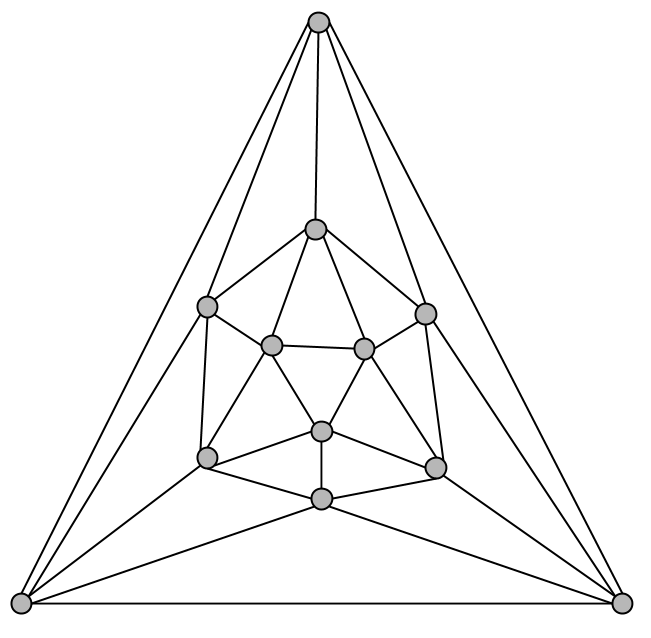
\includegraphics[width=7cm]{iko}
\end{center}
\caption{Der Ikosaeder hat 20 Facetten (gleichseitige Dreiecken), 30 Kanten und 12 Ecken.}
\end{figure}

\begin{figure}[htpb]
\begin{center}
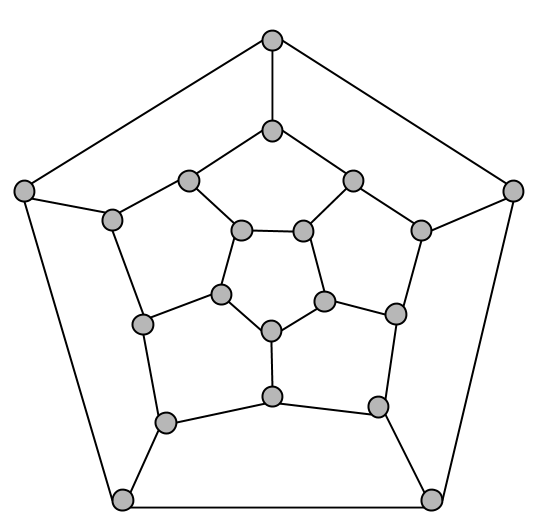
\includegraphics[width=7cm]{dode}
\end{center}
\caption{Der Dodekaeder hat 12 Facetten (regelmäßiges Fünfeck), 30 Kanten und 20 Ecken.}
\end{figure}




\end{task}


\begin{task}{d-dimensionale Polytope}
\item[]

$d$-dimensionaler Einheitswürfel $W_d$\\
\subtask{a}
Geben Sie die Ecken und die $d - 1$-dimensionalen Facetten von $W_d$ an.
Wieviele gibt es davon?
\subtask{b}
Zeichnen Sie den $W_4$ dh. seine Ecken und Kanten möglichst anschaulich.

$d$-dimensionaler Einheitssimplex $S_d$\\
\subtask{a}
Geben Sie die Ecken und die $d - 1$-dimensionalen Facetten von $S_d$ an
Wieviele gibt es davon?
\subtask{b}
Zeichnen Sie den $S_4$ dh. seine Ecken und Kanten möglichst anschaulich.


\end{task}

\begin{task}{Konvexe Hülle}
\item[]

Wir gehen davon aus, dass keine 4 Punkte auf einer Ebene liegen. Die Punkte $p_1, \dots, p_n$ werden nacheinader hinzugefügt. In jedem Schritt wird die konvexe Hülle aktualisiert. Wir nehmen nun an, dass die konvexte Hülle der ersten $k$ Punkte bekannt ist. $p_{k+1}$ kann nun entweder (1) Teil der konvexen Hülle sein, $p_{k+1} \in CH(p_1, \dots, p_n)$ oder (2) außerhalb der konvexen Hülle liegen, $p_{k+1} \not \in CH(p_1, \dots, p_n)$.

Von Punkt $p_{k+1}$ aus gesehen wird $CH(p_1, \dots, p_k)$ in die Ebene projiziert. Es werden Flächen einfügen zwischen allen Kanten die auf dem entstanden Rand $R$ liegen und $p_{k+1}$. Es werden Kanten zwischen allen Knoten auf dem Rand und $p_{k+1}$ hinzufügen. Alle von $p_{k+1}$ sichbaren Flächen werden entfernt.


\begin{algorithm}
\caption{$CH3D(P = \{p_1, p_2, \dots, p_n\})$}
\begin{algorithmic}[1]
\STATE $C \leftarrow CH(p_1, p_2, p_3, p_4)$
\FOR {$i=5$ \TO $n$}
    \IF{$p_i$ liegt außerhalb von $C$}
    \STATE{$R\rightarrow$ Rand durch Projiktion in die Ebene von $p_i$ aus.}
    \FOR {alle Kanten $e \in R$}
        \STATE erzeuge eine neue Facette($e, p_i$)\\
        \STATE erzeuge eine neue Kante(Startpunkt von $e$, $p_i$)\\
    \ENDFOR 
    \ENDIF
\ENDFOR
\end{algorithmic}
\end{algorithm}



\end{task}
\end{document}